% Koma-Script Basisklasse
\documentclass[a4paper,12pt,pagesize,headsepline,bibtotoc,titlepage]{scrartcl}
\usepackage[english]{babel}		% deutsche Trennmuster
\usepackage[utf8]{inputenc}		% direkte Eingabe von Umlauten & Co. (Vorsicht: Encoding im Editor muss auch UTF-8 sein!)

\usepackage[T1]{fontenc}			% T1-Schriften

\usepackage{mathptmx}			% Times/Mathe \rmdefault
\usepackage[scaled=.90]{helvet}	% Skalierte Helvetica \sfdefault
\usepackage{courier}			% Courier \ttdefault

% Zusatzpakete für mehr mathematische Symbole, Einfügen von Grafiken
% und bessere Bildunterschriften
\usepackage{amsmath,amsthm,amsfonts,graphicx,caption}

% Wenn man direkt mit dem pdflatex eine PDF-Datei erzeugt, sollten diese beiden Pakete eingebunden werden
\usepackage{hyperref} % Hyperlinks anklickbar
\usepackage{ae,aecompl} % bessere Bildschirmschriftarten usw.

\pagestyle{headings}

% Abstand der Kopfzeile vom Text:
\headsep4mm

\typearea[current]{current}     % Satzspiegel neu berechnen

% andere Bildunterschrift mit Hilfe von caption
\renewcommand{\figurename}{Abb.}
\renewcommand{\captionlabelfont}{\bf}

\title{
	\includegraphics*[width=0.4\textwidth]{images/hpi_logo.png}\\
	\vspace{24pt}
	Shot Boundary Detection
}
\subtitle{
	Seminar\\
	Practical Video Analyses\\
	Sommersemester 2015
}
\author{
	Tanja Bergmann, Stefan Bunk, Philipp Otto, \\
	Max Reimann, Felix Wolff\\ \\[12pt]
	Betreuer:\\
	Dr. Haojin Yang\\
	Prof. Dr. Christoph Meinel
}
\date{\today}

\begin{document}
\maketitle
\tableofcontents
\newpage

\section{Introduction}
\label{sec:introduction}

Videos and movies are usually built of many independently shot sequences.
In the final videos, these sequences are then cut after each other, which makes the final video.
The goal of \emph{shot boundary detection} is to detect these cuts again, without relying on metadata, solely looking at the frames of the video.
Shot boundary detection is an important preprocessing step for many other video processing, including text recognition, video classification and TODO.

An important distinction is between hard cuts and soft cuts.
Hard cuts are abrupt changes from one frame to another.
Only two frames are involved in a hard-cut, one belong to the ending scene and the other to the starting scene.
Soft cuts are slowly changing from one sequence to another, either by mixing the two sequences frame by frame, or by using other blend effects such as swipes or more creative effects.
Soft cuts can be of arbitrary length, and all frames from the last unchanged frame of the old scene to the first unchanged frame of the new scene are considered part of the soft cut.
Sometimes, even the rate of change (interpolation between two images, or speed of the swipe effect) can change inside a soft cut.
Thus, soft cut detection is the harder task compared to hard cut detection.
TODO: Add illustration.

For humans, shot boundary detection is an easy task.
Computers must rely on changes in color, edges or other approaches based on the raw pixel values.
Especially if the changes are small, e.g. from one dark scene to another, the problem becomes harder for computers.
Humans can still detect cuts in these cases, because they can take the context into account.

This work can be separated in two parts:
First, we present our results for hard cut detection.
TODO: Write some stuff about hard cuts.
Second, we present a new approach to soft cut detection using deep artifical neural networks.
Deep neural networks have seen a rise in popularity in the computer vision community in the last years.
This rise is mostly due to impressive improvements in image classification and video classification tasks.
In this work, we want to automatically learn via artificial neural networks how soft cuts look.
To the best of our knowledge, no one has tried to approach the problem with this approach so far.

The rest of the paper is organized as follows:
Section~\ref{sec:related_work} shows related work for both hard cuts and soft cuts, and gives a short introduction into deep artifical neural networks.
In Section~\ref{sec:hard_cut} we focus on our results for hard cut detection, while Section~\ref{sec:soft_cut} focuses on soft cut detection.
For both we will illustrate, how we preprocessed the given data and evaluated our results.
Finally, in Section~\ref{sec:conclusion} we show, what would be the best steps to improve on our results in future work.

\section{Related Work}
\label{sec:related_work}

\subsection{Shot Boundary Detection}

Many different techniques have been developed for shot boundary detection.
For hard cut detection, a baseline approach compares the change between two frames for each pixel, and sums then up.
Then a threshold is selected: Every value over the threshold is then considered a cut.
However, this approach is prone to error, when there are quick camera movements in the scene, or sudden color changes inside a scene.
Therefore, better approaches have been developed, which are shortly summarized in the next paragraphs.

\paragraph{Color Histograms}
This approach, first used by Zhang~et.al.~\cite{zhang1993automatic} sorts the color values into a histogram with a certain bin size, before comparing the histograms.
Thus, this approach is less prone errors as the baseline approach.
It can compensate for minor changes in the frames.
However, using histograms also means compressing the data, thereby throwing data away.

\paragraph{Luminance Values}
Instead of working on the RGB color space, other color spaces are possible.
Especially luminance values~\cite{petersohn2004fraunhofer}, have shown good performance, as they emphasize the white and black difference.

\paragraph{Edge Detection}
Another approach is to detect the edges in a frame and the subsequent frame.
If the edges differ fundamentally, this is a sign for a hard cut.
In ~\cite{ewerth2005university}, the authors use ``edge histograms of Sobel-filtered (vertically and horizontally) DC-frames''.

\paragraph{Other Techniques}
Other techniques are motion compensation~\cite{}, to prevent false positives from camera movements.
TODO

\paragraph{Machine Learning}
For finding exact thresholds or decision boundaries, many approaches employ machine learning, especially via support vector machines (SVM).
This works by extracing features like histogram bins, edges and then pass these to a machine learning algorithm.
SVMs are popular, because they are ``easy to use and provide a quick classification time after the initial training''~\cite{smeaton2010video}.

It is also possible to combine many of the approaches from above.




\subsection{Deep Neural Networks}
Deep neural networks were very successful in image classification and video classifaction tasks in the last years.

Learning has seen a recent rise in popularity in the computer vision community.
Deep

Image classification, video classification

tagging sequence
RNN/LSTM
enters a sequence


On the contrary, research in shot boundary detection has ceased in the last years.
From 2001 until 2007, the TRECVid~\cite{trecvid} conference series was hosting tracks on shot boundary detection.
The TRECVID committee provided a video test collection with manually annotated gold data, which could be used by different research groups to develop and test their algorithms.
The tasks range from instance detection (e.g. detecting a person in a video), semantic indexing, event detection and many more.
However, as told before, the last challenge for shot boundary detection was in 2007.

We think this decline in research is largely because the current approaches are highly developed, and there is not much potential for further improvements.

This is why we propose to use deep learning approaches for shot boundary detection.
The next sections will detail our approach.


\section{Hard-Cut Detection}
\label{sec:hard_cut}


\subsection{Approach}
\label{sec:hard_cut_approach}

Hard cuts are abrupt transitions from one scene to another.
Normally the contents of the two frames involved in such a cut are highly different, see Figure~\ref{fig:hard_cut_example}, while two consecutive frames in one scene do not differ that much.

\begin{figure}
	\centering
	\includegraphics[scale=.7]{images/hard_cut_example.png}
	\caption{These two consecutive frames form a hard cut.}
	\label{fig:hard_cut_example}
\end{figure}

To detect hard cuts, we therefore want to apply a similarity measure to two subsequent frames.
In our case, we represent frames using their color histograms.
Each frame has three color channels (red, green, blue) and therefore three histograms.
The difference between two frames is then the difference between the histograms.
The histogram difference can be represented as an \emph{3*n}-dimensional vector, where \emph{n} is the number of bins in a color histogram.
So, we are presented with a binary classification task (cut or not) in a \emph{3*n}-dimensional space.

In a next step, the dimensionality can be further reduced by simply adding up the vector elements.
This step is justifiable, since it does not matter which color changed and how much, but the sum of changes in all color channels.
We will evaluate both approaches later. \\
To do the actual classification we train an SVM classifier on a labeled training set.
In our implementation, we use the SVM provided by the OpenCV library\footnote{\url{http://docs.opencv.org/doc/tutorials/ml/introduction_to_svm/introduction_to_svm.html}}.
We transform the input space into a higher dimensional feature space by using a kernelized decision function. The commonly used radial basis function (RBF) kernel is employed:
$$K(x_i,x_j) = exp(-\lambda || x_i - x_j ||^2)$$
where $\lambda$ denotes the width of the kernel and $x_i, x_j $ are vectors from the training set.
This is part of the library.
The complexity parameter C for the soft-margin SVM, as well as other parameters are optimized automatically by using the \emph{train\_auto} method of OpenCVs SVM implementation.
It automatically performs a k-fold cross-validation to choose the best parameter values.

\subsection{Visualization}
\label{sec:hard_cut_visualization}

After having implemented the ideas presented in \ref{sec:hard_cut_approach}, the results were not breathtaking. 
Therefore we wanted to get a feel for the flaws in our approach by visualising the features and the decisions that the SVM made.
To make the visualization explorable and interactive, it is written in \emph{HTML} and \emph{Javascript} using \emph{d3}.
During hard cut detection, we write a \emph{tsv} file containing all required information like the histogram differences, the predicted class and the actual class for every two sequent frames.
This allows us to create the diagram from Figure~\ref{fig:hard_cut_visualization}.

\begin{figure}
	\centering
	\includegraphics[scale=.7]{images/hard_cut_visualization.png}
	\caption{The height of the bars shows the absolute histogram difference. It is calculated by summing up all elements in the histogram difference vector. The color of the bars indicates the decision: green - true positive, gray - true negative, red - false positive, orange - false negative (not in this picture). When hovering over the bars, the actual frames are shown below together with a tooltip containing the file names.}
	\label{fig:hard_cut_visualization}
\end{figure}


THE FOLLOWING MIGHT BE PART OF THE EVALUATION? \\

When inspecting the visualization of a processed video, we can see that the histogram differences are a useful feature for detecting the hard cuts in a video.
In most cases there is one single bar with a very high difference surrounded by very low differences (see green bar in Figure~\ref{fig:hard_cut_visualization}).
However, we can also see some other peaks that are not hard cuts, which are typically surrounded by noisy clusters (Figure~\ref{fig:hard_cut_noise_visualization}).
Those can be soft cut suquences or just rapid changes during one scene.
Since the SVM just takes the difference between two frames into account, it does not "see" the surrounding clusters and therefore makes several mistakes.

\begin{figure}
	\centering
	\includegraphics[scale=.7]{images/hard_cut_noise_visualization.png}
	\caption{The histogram differences are problematic when there is lots of noise between two frames. In this case, a burning fire disturbes the classification and introduces lots of false positives.}
	\label{fig:hard_cut_noise_visualization}
\end{figure}
\subsection{Evaluation}
\label{sec:hard_cut_evaluation}



\section{Soft-Cut Detection}
\label{sec:soft_cut}

\subsection{Data Generation}
\label{sec:soft_cut_data_generation}

The raw data set contains 1,592 soft cut frames and 637,755 non soft cut frames.
% \textcolor{red}{TODO}: Wieviele Softcuts sind es genau? Das ist vllt die spannendere Zahl.
This is a highly imbalanced ratio, which impedes the training.
To achieve a good generalization of a recurrent neural net, we determined that more data was necessary.
% \textcolor{red}{TODO}: Hier muss ein Zitat/Referenz stehen, das man bei DL viel Data braucht.
For that, we generated more data by blending random sequences into each other.
The procedure for generating a new random sequence works as follows:
First, we randomly pick two subsequent cuts from the gold standard, each with a start and end frame respectively.
Between the end frame of the first cut and the start frame of the next cut, we can randomly select a subsequence with the desired transition length.
This way, it is guaranteed that there is no hard cut or soft cut in the random sequence we picked.
Afterwards, we repeat this process with two other random cuts.
As the result, we now have two randomly selected sequences of the same length, which we can now blend into each other.
In order to blend two random sequences, we have multiple options for tweening behaviour.
The standard tweening function is linear, but we also used ease-in, ease-out, and others, see Figure~\ref{fig:data_generation}.
The tweening function is randomly selected, as well.
As the transition type we use a classic \textit{dissolve}.

In order to achieve further variance in the generated data, we flip the two sequences randomly at the x- or y-axis or at both axes.
With this approach we generated about 50 GB of data.
% \textcolor{red}{TODO}: Das ist ja jetzt gerade unvergleichbar mit den Zahlen von oben, weil wir oben absolute Zahlen hatten und hier auf einmal GB.
% Das muessen wir noch vereinheitlichen.
% ICh bin dafuer, hier noch die Anzahl der Soft cuts/non soft cuts hinzuschreiben.

\begin{figure}
    \centering
    \includegraphics[scale=.5]{images/data_generation.jpg}
    \caption{}
    \label{fig:data_generation}
\end{figure}
% \textcolor{red}{TODO}: Figure Text missing.

\subsection{Approach}
\label{sec:soft_cut_approach}

For the soft cut detection we decided to use a deep learning approach.
More concrete we used the RNN/LSTM implementation by Jeff Donahue\footnote{\url{https://github.com/BVLC/caffe/pull/2033}}. \\
This RNN/LSTM implementation takes two different inputs: On the one hand the raw pixel values and on the other hand a tagging sequence.
A tagging seuqence represents sequences of frames, where one sequence of frames might represent a soft cut in our case.
Using this implementation allows us to incorporate the information of a frame, which is at the beginning of a frame sequence, to a frame, which is located later in the same sequence.
So the net memorizes previous decision along a sequence of frames. \\
But using this architecture has one problem, as stated by Jeff Donahue: `"backpropagation [through the LSTM] is truncated along the batch boundaries'" [TODO: Quelle].
So one or more frame sequences has to fit exactly into the batch size used by the RNN/LSTM.
This is hard to archive if we want to use variable length of frame sequences.
Therefore we decided to use a fixed size for the sequences of frames in a tagging sequence, i.e. we only check for example 10 consecutive frames of being a soft cut or not.  \\
However, we still want to find soft cut of arbitrary length in a video.
To achieve this, we repeatedly test fixed-size frame sequences.

\begin{figure}[!htb]
	\centering
	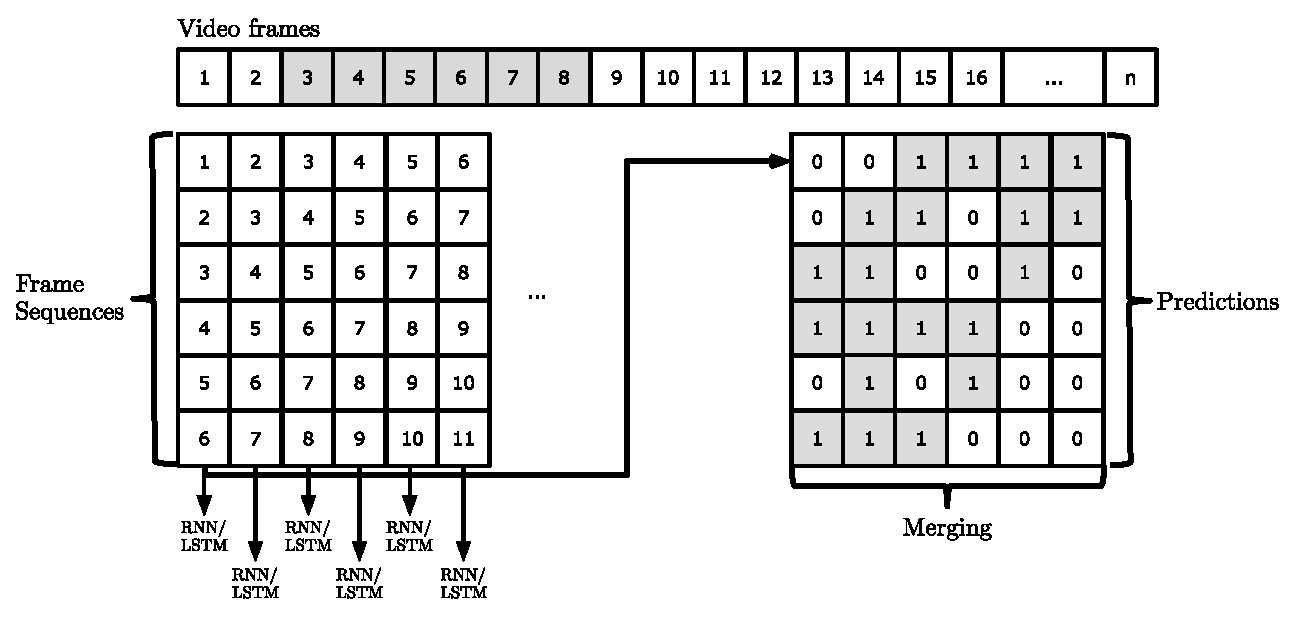
\includegraphics[scale=.7]{images/soft_cut_approach.eps}
	\caption{To classify soft cuts of arbitrary length, we repeatedly test fixed-size frame sequences. In this example we test sequences of size six. Afterwards the predictions given by the RNN/LSTM are merged, so that we have one prediction per frame.}
	\label{fig:soft_cut_approach}
\end{figure}

 has to fit into the batch size.



When classifying a soft cut sequence, the result is one prediction per frame.
We therefore applied several strategies for combining the per-frame result to get one per-sequence result.

\subsection{Evaluation}
\label{sec:hard_cut_evaluation}



\section{Conclusion}
\label{sec:conclusion}

What went wrong:
More data?

In summary.
We still think, that the soft cut detection could be solved with deep learning.
However, the basic approach with using a recurrent neural network does not work.
More work and innovation is required in this area.

We think that the main problem is, that the convolutional network cannot really learn good features, because there is nothing characteristic about a soft cut frame.



\newpage
\begin{thebibliography}{1}

\bibitem{meinel2008}
C.~Meinel.
``Tele-Lab IT-Security: an Architecture for an online virtual IT Security Lab'',
\emph{International Journal of Online Engineering (iJOE)},
X, 2008.

\end{thebibliography}

\end{document}